\section{Heurística de búsqueda local}

% Obviamente, el Doc está en desacuerdo y dice que la heurística golosa no es
% la mejor idea. Para justificar su postura les pide diseñar e implementar una
% heurística de búsqueda local para MCS, y desarrollar los siguientes puntos
% para, de una buena vez, convencer a Marty:
% a) Explicar detalladamente el algoritmo implementado. Plantear al menos dos
%    vecindades distintas para la búsqueda.
% b) Calcular el orden de complejidad temporal de peor caso de una iteración
%    del algoritmo de búsqueda local (para las vecindades planteadas). Si es
%    posible, dar una cota superior para la cantidad de iteraciones de la
%    heurística.
% c) Realizar una experimentación que permita observar la performance del
%    algoritmo comparando los tiempos de ejecución y la calidad de las
%    soluciones obtenidas, en función de las vecindades utilizadas y elegir,
%    si es posible, la configuración que mejores resultados provea para el
%    grupo de instancias utilizado.

\subsection{Introducción}
Este ejercicio consiste en la implementación de una heurística de búsqueda
local para el problema de \acr{MCS}, que sea capaz de iterar sobre una
solución dada y mejorarla en búsqueda de óptimos locales.

Al igual que en el ejercicio anterior, asumiremos sin pérdida de generalidad
que los grafos $G_1$ y $G_2$ para los que quiere resolverse el problema son
tales que $N_1 \leq N_2$, siendo $N_1$ y $N_2$ sus cantidades de nodos
respectivas.

\subsection{Vecindades planteadas}

El principal elemento a definir a la hora de plantear una heurística de
búsqueda local es qué soluciones se considerarán vecinas. Es decir, es
necesario plantear una \emph{relación de vecindad} entre el espacio de
soluciones del problema. Para esto, será útil adoptar de nuevo el enfoque
de ver a una solución de \acr{MCS} como un mapeo $s : V(G_1) \to V(G_2)$.
De esta forma, se define el espacio de soluciones posibles del problema como
\[ S = \lbrace s : V(G_1) \to V(G_2) \ \vert\ s \text{ es inyectiva}
\rbrace \]
y se plantean dos alternativas para definir una relación simétrica $N
\subseteq S \times S$.
Luego, dada una solución del problema $s \in S$, la heurística
explorará todas las soluciones vecinas de $s$, es decir, aquellas que se
relacionen con $s$ a través de $N$.

Una característica que se tuvo en cuenta a la hora de definir las vecindades
fue que cualquier solución fuera alcanzable desde cualquier otra, moviéndose
sucesivas veces entre soluciones vecinas.

A continuación se describen las dos vecindades planteadas, junto con el
pseudocódigo del algoritmo que itera sobre cada una de ellas y selecciona,
dada una solución cualquiera, la mejor entre sus soluciones vecinas. También
se calcula, en cada caso, una cota teórica para la complejidad de dicho
algoritmo. Para esto se tienen en cuenta las estructuras utilizadas al
implementarlo; muchas de las operaciones que se consideran $\ord(1)$ lo son en
realidad al considerar el costo amortizado, dado que varios de los mapeos
necesarios se implementan mediante tablas de \emph{hash}.

\subsubsection{Vecindad I}
Dos soluciones $s, s' \in S$ se consideran vecinas en la vecindad I
si $s'$ es el resultado de modificar el mapeo de exactamente uno de los nodos
de $G_1$ en $s$, asignándole un nodo de $G_2$ que esté libre en $s$. Es
decir, $(s, s') \in N_1$ si y solo si
\begin{itemize}
    \item $(\exists \ v \in G_1)\ s(v) \neq s'(v)$, y
    \item $(\forall \ w \in G_1)\ w \neq v \Rightarrow s(w) = s'(w)$.
\end{itemize}

Es importante notar que esta vecindad no está bien definida, y por lo tanto no
puede aplicarse, si $\#V(G_1) = \#V (G_2)$.

\begin{figure}[htbp]
    \centering
    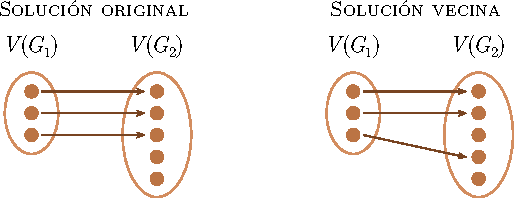
\includegraphics{imagenes/ex5_vecindad1.pdf}
    \caption{Ejemplo de soluciones vecinas que es posible obtener mediante la
    vecindad I.}
    \label{fig:ej5:vecindad1}
\end{figure}

\subheading{Pseudocódigo de una iteración}

\begin{algorithm}[H]
    \SetAlgoVlined
    \caption{Iteración de la vecindad I}
    \Input{Dos grafos $G_1$ y $G_2$, con $\#V(G_1) < \#V(G_2)$, y un tercer
    grafo \textit{solución}, cuyos nodos son pares de $V(G_1) \times V(G_2)$,
    representando la solución a \acr{MCS} que se pretende mejorar. Este último
    grafo será modificado por el algoritmo.}
    \Output{Un valor de verdad indicando si se pudo mejorar la solución.}
    \textit{hay\_mejora} $\gets$ \textsf{falso} \;
    \textit{mejor\_diferencia\_aristas} $\gets$ 0 \;

    \ForEach{vértice $(v, w)$ de \textit{solución}} {
        \ForEach{vértice $w'$ de $G_2$ que no esté en el mapeo} {
            \textit{cant\_aristas\_perdidas} $\gets$ grado de $(v, w)$ en \textit{solución} \;
            \textit{aristas\_nuevas} $\gets$ vector vacío \;
            \ForEach {vecino $\tilde{w}$ de $w_2$ en $G_2$} {
                \If{$\tilde{w}$ está en el mapeo} {
                    $\tilde{v}$ $\gets$ nodo de $G_1$ al que está mapeado $\tilde{w}$ \;
                    \If{$\tilde{v}$ es vecino de $v$ en $G_1$} {
                        agregar $(\tilde{v}, \tilde{w})$ a \textit{aristas\_nuevas} \;
                    }
                }
            }
            \textit{diferencia\_aristas} $\gets$ $\vert$\textit{aristas\_nuevas}$\vert$
                $-$ \textit{cant\_aristas\_perdidas} \;
            \If{\textit{diferencia\_aristas} $>$ \textit{mejor\_diferencia\_aristas}} {
                \textit{hay\_mejora} $\gets$ \textsf{verdadero} \;
                \textit{mejor\_diferencia\_aristas} $\gets$ \textit{diferencia\_aristas} \;
                \textit{mejor\_para\_eliminar} $\gets$ $(v, w)$ \;
                \textit{mejor\_para\_agregar} $\gets$ $(v, w')$ \;
                \textit{mejor\_aristas\_nuevas} $\gets$ \textit{aristas\_nuevas} \;
            }
        }
    }
    \eIf{\textit{hay\_mejora}} {
        eliminar el nodo \textit{mejor\_para\_eliminar} de \textit{solución} \;
        agregar el nodo \textit{mejor\_para\_agregar} a \textit{solución} \;
        \ForEach{par $(\tilde{v}, \tilde{w})$ en \textit{mejor\_aristas\_nuevas}} {
            agregar en \textit{solución} una arista entre
                \textit{mejor\_para\_agregar} y $(\tilde{v}, \tilde{w})$ \;
        }
        \Return{\textsf{verdadero}}
    } {
        \Return{\textsf{falso}}
    }
\end{algorithm}

\subheading{Complejidad temporal}

Cada iteración del algoritmo recorre la vecindad completa de la solución que
se busca mejorar; para esto se utilizan dos ciclos anidados. El primero de
ellos recorre todos los nodos de la solución, es decir, realiza $N_1$
iteraciones. El ciclo interior recorre el conjunto $W_U \subseteq G_2$ de los
nodos de $G_2$ que no forman parte del mapeo, que tiene $N_2 - N_1$ elementos.
Dentro de este ciclo, además de realizarse operaciones con un costo constante,
se itera a su vez, para cada nodo $w \in W_U$, sobre el conjunto de sus
vecinos, cuyo cardinal es $\deg(w)$. Para cada uno de estos vecinos se
verifica si pertenece al mapeo y, en caso afirmativo, debe decidirse si son
adyacentes en $G_1$ los nodos mapeados a $w$ y su vecino en cuestión. Esto
último tiene complejidad $\ord(\deg(v))$, siendo $v$ el nodo de $G_1$
mapeado a $w$, que puede acotarse por $\ord(N_1)$. De todo lo anterior se
concluye que la complejidad del primer ciclo es:

\begin{align*}
\ord\left( N_1 \times \left( \sum_{w \in W_U} \left(1 + \deg(w) \times N_1
\right) \right) \right)
&= \ord \left( N_1 \times \left( (N_2 - N_1) + N_1 \times \sum_{W \in W_U}
\deg(w) \right) \right) \\
&= \ord \left( N_1 \times \left( (N_2 - N_1) + N_1 \times \sum_{w \in V(G_2)}
\deg(w) \right) \right) \\
&= \ord \left( N_1 \times \left( (N_2 - N_1) + N_1 \times M_2 \right) \right) \\
&= \ord \left( N_1 \times (N_2 - N_1) + N_1^2 \times M_2 \right)
\end{align*}

En la segunda parte del algoritmo, si se encontró alguna mejora a la solución,
deben modificarse las estructuras que se utilizan para almacenar la misma. En
primer lugar se elimina un nodo de la solución; el costo de esta operación es
el grado de dicho nodo. Dado que todas las aristas adyacentes a un nodo de la
solución deben corresponderse con aristas en $G_1$, el grado máximo de un nodo
en la solución está acotado por el grado máximo de un nodo de $G_1$, que es
$N_1 - 1$. Luego se agrega a la solución un nuevo nodo; esto tiene un costo de
orden $\ord(N_2 - N_1)$, ya que debe eliminarse el vértice de un vector que
almacena los nodos que no pertenecen al mapeo. Por último se incorporan, cada
una con un costo constante, todas las aristas correspondientes al nuevo nodo,
cuya cantidad está igualmente acotada por $N_1 - 1$.

De esta forma, la segunda parte de la iteración tiene un costo de $\ord(N_2 -
N_1) + \ord(N_1) = \ord (N_1 + N_2)$, que resulta absorbido por el costo de
recorrer la vecindad, obteniendo una complejidad total para cada iteración de
\[ \ord \left( N_1 \times (N_2 - N_1) + N_1^2 \times M_2 \right) \]

\subsubsection{Vecindad II}
Dos soluciones $s, s' \in S$ se consideran vecinas en la vecindad II
si $s'$ es el resultado de aplicar sobre $s$ alguno de estos cambios:
\begin{itemize}
    \item \textsc{Permutación:} permutar los mapeos de dos nodos de $G_1$, de
    forma tal que $s'(v_1) = s(v_2)$ y $s'(v_2) = s(v_1)$. Formalmente,
    \begin{itemize}
        \item $(\exists \ v_1, v_2 \in G_1)\ s'(v_1) = s(v_2)$ y $s'(v_2) = s
        (v_1)$, y
        \item $(\forall \ w \in G_1)\ w \neq v_1$ y $w \neq v_2
        \Rightarrow s(w) = s'(w)$.
    \end{itemize}
    \item \textsc{Intercambio:} la misma operación que define la vecindad
    I, es decir, modificar el mapeo de exactamente uno de los nodos
    de $G_1$, asignándole un nodo de $G_2$ que esté libre en $s$. Formalmente,
    \begin{itemize}
        \item $(\exists \ v \in G_1)\ s(v) \neq s'(v)$, y
        \item $(\forall \ w \in G_1)\ w \neq v \Rightarrow s(w) = s'(w)$.
    \end{itemize}
\end{itemize}

La vecindad II no tiene problemas de definición en el caso de que $\#V(G_1)
= \#V (G_2)$.

\begin{figure}[htbp]
    \centering
    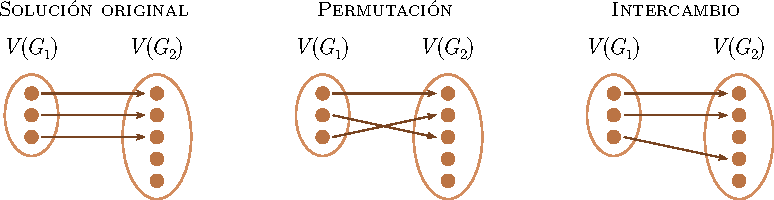
\includegraphics{imagenes/ex5_vecindad2.pdf}
    \caption{Soluciones vecinas que es posible obtener mediante la vecindad
    II.}
    \label{fig:ej5:vecindad2}
\end{figure}

Cabe destacar que la vecindad I está contenida en la vecindad II,
siendo esta última considerablemente más grande. Desde un punto de vista
computacional, esto tiene como desventaja inmediata un mayor costo a la hora
de recorrer y explorar la vecindad, pero corre con la ventaja de que resulta
posible pasar de una solución dada a cualquier otra en una cantidad de
iteraciones menor (se puede decir que $N_2$ es una vecindad más
\emph{densamente conectada} que I).

\subheading{Pseudocódigo de una iteración}

\begin{algorithm}[H]
    \SetAlgoVlined
    \caption{Iteración de la vecindad II}
    \Input{Dos grafos $G_1$ y $G_2$, con $\#V(G_1) < \#V(G_2)$, y un tercer
    grafo \textit{solución}, cuyos nodos son pares de $V(G_1) \times V(G_2)$,
    representando la solución a \acr{MCS} que se pretende mejorar. Este último
    grafo será modificado por el algoritmo.}
    \Output{Un valor de verdad indicando si se pudo mejorar la solución.}
    \textit{hay\_mejora} $\gets$ \textsf{falso} \;
    \textit{mejor\_diferencia\_aristas} $\gets$ 0 \;

    \ForEach{vértice $w_1$ de $G_2$} {
        \ForEach{vértice $w_2$ de $G_2$} {
            \textit{diferencia\_aristas} $\gets$ $0$ \;
            \uIf{$w_1$ y $w_2$ están en el mapeo} {
                (Código extraido como Algoritmo \ref{alg:ej5:vec2:permutacion})
            }
            \ElseIf{$w_1$ está en el mapeo o $w_2$ está en el mapeo} {
                (Código extraido como Algoritmo \ref{alg:ej5:vec2:intercambio})
            }
            \If{\textit{diferencia\_aristas} $>$ \textit{mejor\_diferencia\_aristas}} {
                \textit{hay\_mejora} $\gets$ \textsf{verdadero} \;
                \textit{mejor\_diferencia\_aristas} $\gets$ \textit{diferencia\_aristas} \;
                \textit{mejor\_acción} $\gets$ \textit{acción} \;
                \textit{mejor\_1} $\gets$ $(v_1, w_1)$ \;
                \textit{mejor\_2} $\gets$ $(v_2, w_2)$ \;
                \textit{mejor\_aristas\_nuevas\_1} $\gets$ \textit{aristas\_nuevas\_1} \;
                \textit{mejor\_aristas\_nuevas\_2} $\gets$ \textit{aristas\_nuevas\_2} \;
            }
        }
    }
    \eIf{\textit{hay\_mejora}} {
        \uIf{\textit{mejor\_acción} $=$ \textsf{permutación}} {
            eliminar los nodos \textit{mejor\_1} y \textit{mejor\_2} de \textit{solución} \;
            \textit{nuevo\_1} $\gets$ (\textit{mejor\_1}.primero, \textit{mejor\_2}.segundo) \;
            \textit{nuevo\_2} $\gets$ (\textit{mejor\_2}.primero, \textit{mejor\_1}.segundo) \;
            agregar los nodos \textit{nuevo\_1} y \textit{nuevo\_2} a \textit{solución}\;
            \If {\textit{mejor\_1} y \textit{mejor\_2} eran adyacentes en \textit{solución}} {
                agregar en \textit{solución} una arista entre \textit{mejor\_1} y \textit{mejor\_2} \;
            }
            \ForEach{par $(\tilde{v}, \tilde{w})$ en \textit{mejor\_aristas\_nuevas\_1}} {
                agregar en \textit{solución} una arista entre
                    \textit{mejor\_1} y $(\tilde{v}, \tilde{w})$ \;
            }
            \ForEach{par $(\tilde{v}, \tilde{w})$ en \textit{mejor\_aristas\_nuevas\_2}} {
                agregar en \textit{solución} una arista entre
                    \textit{mejor\_2} y $(\tilde{v}, \tilde{w})$ \;
            }
        }
        \ElseIf{\textit{mejor\_accion} $=$ \textsf{intercambio}} {
            eliminar el nodo \textit{mejor\_1} de \textit{solución} \;
            agregar el nodo \textit{mejor\_2} a \textit{solución} \;
            \ForEach{par $(\tilde{v}, \tilde{w})$ en \textit{mejor\_aristas\_nuevas\_1}} {
                agregar en \textit{solución} una arista entre
                    \textit{mejor\_1} y $(\tilde{v}, \tilde{w})$ \;
            }
        }
        \Return{\textsf{verdadero}}
    } {
        \Return{\textsf{falso}}
    }
\end{algorithm}
\bigskip

\begin{algorithm}[H]
    \SetAlgoVlined
    \caption{Iteración de la vecindad II (Sección correspondiente a la acción \textsc{Permutación})}
    \label{alg:ej5:vec2:permutacion}
    \textit{acción} $\gets$ \textsf{permutación} \;
    $v_1$ $\gets$ nodo de $G_1$ al que está mapeado $w_1$ \;
    $v_2$ $\gets$ nodo de $G_1$ al que está mapeado $w_2$ \;
    \textit{cant\_aristas\_perdidas} $\gets$ (grado de $(v_1, w_1)$ en \textit{solución}) +
        (grado de $(v_2, w_2)$ en \textit{solución}) \;
    \If{$(v_1, w_1)$ es adyacente a $(v_2, w_2)$ en \textit{solución}} {
        \textit{cant\_aristas\_perdidas} $\gets$ \textit{cant\_aristas\_perdidas} $-$ $2$ \;
    }
    \textit{aristas\_nuevas\_1} $\gets$ vector vacío \;
    \ForEach{vecino $\tilde{w}$ de $w_1$ en $G_2$} {
        \If{$\tilde{w} \neq w_2$ y $\tilde{w}$ está en el mapeo} {
            $\tilde{v}$ $\gets$ nodo de $G_1$ al que está mapeado $\tilde{w}$ \;
            \If{$\tilde{v}$ es vecino de $v_1$ en $G_1$} {
                agregar $(\tilde{v}, \tilde{w})$ a \textit{aristas\_nuevas\_1} \;
            }
        }
    }
    \textit{aristas\_nuevas\_2} $\gets$ vector vacío \;
    \ForEach{vecino $\tilde{w}$ de $w_2$ en $G_2$} {
        \If{$\tilde{w} \neq w_1$ y $\tilde{w}$ está en el mapeo} {
            $\tilde{v}$ $\gets$ nodo de $G_1$ al que está mapeado $\tilde{w}$ \;
            \If{$\tilde{v}$ es vecino de $v_2$ en $G_1$} {
                agregar $(\tilde{v}, \tilde{w})$ a \textit{aristas\_nuevas\_2} \;
            }
        }
    }
    \textit{diferencia\_aristas} $\gets$ $\vert$\textit{aristas\_nuevas\_1}$\vert$ $+$
        $\vert$\textit{aristas\_nuevas\_2}$\vert$ $-$ \textit{cant\_aristas\_perdidas} \;
\end{algorithm}
\bigskip

\begin{algorithm}[H]
    \SetAlgoVlined
    \caption{Iteración de la vecindad II (Sección correspondiente a la acción \textsc{Intercambio})}
    \label{alg:ej5:vec2:intercambio}
    \textit{acción} $\gets$ \textsf{intercambio} \;
    \If{$w_1$ no forma parte del mapeo} {
        llamar $w_1$ a $w_2$ y viceversa (para poder asumir
            que $w_1$ es el nodo que está mapeado) \;
    }
    $v_1$ $\gets$ nodo de $G_1$ al que está mapeado $w_1$ \;
    $v_2$ $\gets$ $v_1$ \;
    \textit{cant\_aristas\_perdidas} $\gets$ grado de $(v_1, w_1)$ en \textit{solución} \;
    \textit{aristas\_nuevas\_1} $\gets$ vector vacío \;
    \ForEach {vecino $\tilde{w}$ de $w_2$ en $G_2$} {
        \If{$\tilde{w}$ está en el mapeo} {
            $\tilde{v}$ $\gets$ nodo de $G_1$ al que está mapeado $\tilde{w}$ \;
            \If{$\tilde{v}$ es vecino de $v_1$ en $G_1$} {
                agregar $(\tilde{v}, \tilde{w})$ a \textit{aristas\_nuevas\_1} \;
            }
        }
    }
    \textit{diferencia\_aristas} $\gets$ $\vert$\textit{aristas\_nuevas}$\vert$
        $-$ \textit{cant\_aristas\_perdidas} \;
\end{algorithm}

\subheading{Complejidad temporal}

Dado que el tamaño de esta vecindad es mayor al de la otra alternativa
planteada, también será más costosa cada iteración que deba explorarla. El
recorrido se hace mediante dos ciclos anidados, cada uno de los cuales se
repite $N_2$ veces. De esta forma se recorren todos los pares posibles de
dos nodos de $G_2$. No obstante, debido a que según el caso el código que se
ejecuta en cada una de estas repeticiones es diferente, se estudiará la
complejidad de cada uno de ellos por separado.

\begin{itemize}
    \item La operación de \emph{permutación} se realiza cuando se
    selecciona un par de nodos distintos $w_1, w_2$ de $W_M \subseteq G_2$,
    siendo $W_M$ el conjunto de los nodos que pertenecen al mapeo (cuyo
    cardinal es $N_1$). Como la cantidad de estos nodos es $N_1$, este tipo de
    iteración se ejecuta $\ord(N_1^2)$ veces. Además de operaciones con costo
    constante, dentro de cada repetición de este proceso se ejecutan dos
    ciclos, uno de los cuales itera sobre los vecinos de $w_1$ ($\deg(w_1)$) y
    el otro, sobre los vecinos de $w_2$ ($\deg(w_2)$). Para cada uno de ellos
    se chequea su adyacencia en $G_1$ con los nodos mapeados a $w_1$ y $w_2$,
    respectivamente, lo cual tiene un costo acotable por $\ord(N_1)$.

    Es importante notar que el primer ciclo se ejecutará exactamente $N_1 - 1$
    veces para cada posible $w_1$, y análogamente el segundo se ejecutará
    exactamente $N_1 - 1$ veces para cada posible $w_2$. Así, la complejidad
    combinada de estas iteraciones, considerando por separado las operaciones
    constantes y los dos ciclos mencionados, será de
    \begin{align*}
    \ord & \left( N_1^2 + N_1 \times \sum_{w_1 \in W_M} ((1 +
    \deg(w_1)) \times N_1) + N_1 \times \sum_{w_2 \in W_M} ((1 + \deg(w_2))
    \times N_1) \right) \\
    &= \ord \left( N_1^2 + 2 \times N_1 \times \sum_{w \in W_M} ((1 +
    \deg(w)) \times N_1) \right) \\
    &= \ord \left( N_1^2 + 2 \times N_1 \times \left( N_1 + N_1 \times \sum_{w
    \in V(G_2)} \deg(w) \right) \right) \\
    &= \ord \left( N_1^2 + 2 \times N_1 \times \left( N_1 + N_1 \times M_2
    \right) \right) \\
    &= \ord \left( N_1^2 + 2 \times N_1^2 \times \left( 1 + M_2 \right) \right) \\
    &= \ord (N_1^2 \times (1 + M_2))
    \end{align*}

    \item La operación de \emph{intercambio} se realiza cuando se selecciona
    un nodo de $G_2$ perteneciente al mapeo y otro que no está en el mismo.
    Dado que hay $N_1$ de los primeros y $N_2 - N_1$ de los
    segundos, este tipo de iteración se realiza $(N_1) \times (N_2 - N_1)$
    veces. El código que se ejecuta en estos casos es muy similar al de la
    vecindad I, y la cota teórica que se obtiene para la complejidad de todas
    ellas en su conjunto es idéntica a la de ese caso, es decir,
    $\ord \left( N_1 \times (N_2 - N_1) + N_1^2 \times M_2 \right)$.

    \item Cuando se selecciona un par que contiene dos nodos que no están en
    el mapeo, o que contiene dos veces a un nodo del mapeo, se omite dicho
    par, con un costo $\ord(1)$. Hay un total de $N_1 + (N_2 - N_1)^2$ de
    estas iteraciones.
\end{itemize}

Sumando la complejidad de los tres tipos de iteraciones recién descriptos, se
obtiene una complejidad total para la primera etapa del algoritmo de
$\ord \left( N_1^2 \times (1 + M_2) + N_1 \times N_2 + (N_2 - N_1)^2 \right)$.

Por su parte, la segunda etapa del algoritmo, que se ejecuta si la
iteración produjo alguna mejora, aplicando estos cambios a las estructuras
que almacenan la solución, dependerá de si la mejora encontrada proviene de
realizar una \emph{permutación} o un \emph{intercambio}. En el segundo
caso las operaciones que se realizan son las mismas que en la segunda etapa
de la vecindad I, mientras que en el primer caso son muy similares, solo que
deben agregarse dos nodos en lugar de uno. En ambos casos la complejidad es la
misma, $\ord (N_1 + N_2)$, que al igual que en la otra vecindad resulta
absorbida por el costo de la primera parte del algoritmo. De esta forma, la
complejidad total de una iteración de la vecindad II tiene un costo
\[
\ord \left( N_1^2 \times (1 + M_2) + N_1 \times N_2 + (N_2 - N_1)^2 \right)
\]


\subsection{Experimentación}

	Dadas ciertas familias de grafos (arboles, ciclos, completos y bipartos) y distintos tamaños de grafos ($\#(g_1)$ $n$ veces mas que $\#(g_2)$, variando el $n$ entre 1 y $\#(g_2)$), se querra comparar, cuanto mejor que la solución greedy es el local search, cual de las dos vecindades es mejor, que porcentaje de vencindad a mirar da un mejor resultado y a partir de cuantas iteraciones empieza a agragar pocas ó deja de agregar arristas.


	\subsubsection{Porcentaje de vencindad optimo}

	Dadas familias con orden $n$(tree, ciclo) de arristas y orden $n^2$,(bipartito, completo) se varia el porcentaje de vecindad a mirar en cada iteración.


    \subheading{Primera vecindad}



    \begin{figure}[H]
        \centering
        \begin{tikzpicture}
            \begin{axis}[
                    title={},
                    xlabel={Porcentaje de vecindad a mirar en cada iteración.},
                    ylabel={Cantidad de arristas promedio},
                    scaled x ticks=false,
                    scaled y ticks=false,
                    enlargelimits=0.05,
                    width=0.5\textwidth,
                    height=0.5\textwidth,
                    legend pos=north west,
                    legend cell align=left,
                    xmin=0
                ]

                \addplot[color=black] table[x index=0,y index=1]{../exp/ej5/big_tree_vs_small_cicle_neighbourhood_1_proportion};

                \legend{$T_{M}$}
            \end{axis}
        \end{tikzpicture}
        \caption{$g_1$ es un ciclo de 300 nodos y $g_2$ es un random tree de 600 .}
        \label{fig:exp5:var-pym-base}
    \end{figure}

    \begin{figure}[H]
        \centering
        \begin{tikzpicture}
            \begin{axis}[
                    title={},
                    xlabel={Porcentaje de vecindad a mirar en cada iteración.},
                    ylabel={Cantidad de arristas promedio},
                    scaled x ticks=false,
                    scaled y ticks=false,
                    enlargelimits=0.05,
                    width=0.5\textwidth,
                    height=0.5\textwidth,
                    legend pos=north west,
                    legend cell align=left,
                    xmin=0
                ]

                \addplot[color=black] table[x index=0,y index=1]{../exp/ej5/big_cicle_vs_small_tree_1_proportion};

                \legend{$T_{M}$}
            \end{axis}
        \end{tikzpicture}
        \caption{$g_1$ es un random tree de 300 nodos y $g_2$ es un ciclo de 600.}
        \label{fig:exp5:var-pym-base}
    \end{figure}


    \begin{figure}[H]
        \centering
        \begin{tikzpicture}
            \begin{axis}[
                    title={},
                    xlabel={Porcentaje de vecindad a mirar en cada iteración.},
                    ylabel={Cantidad de arristas promedio},
                    scaled x ticks=false,
                    scaled y ticks=false,
                    enlargelimits=0.05,
                    width=0.5\textwidth,
                    height=0.5\textwidth,
                    legend pos=north west,
                    legend cell align=left,
                    xmin=0
                ]

                \addplot[color=black] table[x index=0,y index=1]{../exp/ej5/big_bipartite_some_edges_vs_big_tree_neighbourhood_1_proportion};

                \legend{$T_{M}$}
            \end{axis}
        \end{tikzpicture}
        \caption{$g_1$ es un bipartito  300 nodos con promedio de arristas de $0.5$ y  $g_2$ es un random tree de 600.}

        \label{fig:exp5:var-pym-base}
    \end{figure}

      \begin{figure}[H]
        \centering
        \begin{tikzpicture}
            \begin{axis}[
                    title={},
                    xlabel={Porcentaje de vecindad a mirar en cada iteración.},
                    ylabel={Cantidad de arristas promedio},
                    scaled x ticks=false,
                    scaled y ticks=false,
                    enlargelimits=0.05,
                    width=0.5\textwidth,
                    height=0.5\textwidth,
                    legend pos=north west,
                    legend cell align=left,
                    xmin=0
                ]

                \addplot[color=black] table[x index=0,y index=1]{../exp/ej5/big_bipartite_some_edges_vs_big_cicle_neighbourhood_1_proportion};


                \legend{$T_{M}$}
            \end{axis}
        \end{tikzpicture}
        \caption{$g_1$ es un bipartito  300 nodos con promedio de arristas de $0.5$ y $g_2$ es un ciclo de 600.}

        \label{fig:exp5:var-pym-base}
    \end{figure}

    \begin{figure}[H]
        \centering
        \begin{tikzpicture}
            \begin{axis}[
                    title={},
                    xlabel={Porcentaje de vecindad a mirar en cada iteración. },
                    ylabel={Cantidad de arristas promedio},
                    scaled x ticks=false,
                    scaled y ticks=false,
                    enlargelimits=0.05,
                    width=0.5\textwidth,
                    height=0.5\textwidth,
                    legend pos=north west,
                    legend cell align=left,
                    xmin=0
                ]

                \addplot[color=black] table[x index=0,y index=1]{../exp/ej5/big_bipartite_some_edges_vs_small_complete_neighbourhood_2_proportion};

                \legend{$T_{M}$}
            \end{axis}
        \end{tikzpicture}
        \caption{$g_1$ es un bipartito  300 nodos con promedio de arristas de $0.5$ y $g_2$ es un completo de 150.}

        \label{fig:exp5:var-pym-base}
    \end{figure}


    \subheading{Segunda Vecindad}

    \begin{figure}[H]
        \centering
        \begin{tikzpicture}
            \begin{axis}[
                    title={},
                    xlabel={Porcentaje de vecindad a mirar en cada iteración. },
                    ylabel={Cantidad de arristas promedio},
                    scaled x ticks=false,
                    scaled y ticks=false,
                    enlargelimits=0.05,
                    width=0.5\textwidth,
                    height=0.5\textwidth,
                    legend pos=north west,
                    legend cell align=left,
                    xmin=0
                ]

                \addplot[color=black] table[x index=0,y index=1]{../exp/ej5/big_tree_vs_small_cicle_neighbourhood_2_proportion};

                \legend{$T_{M}$}
            \end{axis}
        \end{tikzpicture}
        \caption{$g_1$ es un ciclo de 300 nodos y $g_2$ es un random tree de 600.}
        \label{fig:exp5:var-pym-base}
    \end{figure}

    \begin{figure}[H]
        \centering
        \begin{tikzpicture}
            \begin{axis}[
                    title={},
                    xlabel={Porcentaje de vecindad a mirar en cada iteración.},
                    ylabel={Cantidad de arristas promedio},
                    scaled x ticks=false,
                    scaled y ticks=false,
                    enlargelimits=0.05,
                    width=0.5\textwidth,
                    height=0.5\textwidth,
                    legend pos=north west,
                    legend cell align=left,
                    xmin=0
                ]

                \addplot[color=black] table[x index=0,y index=1]{../exp/ej5/big_cicle_vs_small_tree_2_proportion};

                \legend{$T_{M}$}
            \end{axis}
        \end{tikzpicture}
        \caption{$g_1$ es un random tree de 300 nodos y $g_2$ es un ciclo de 600.}
        \label{fig:exp5:var-pym-base}
    \end{figure}


    \begin{figure}[H]
        \centering
        \begin{tikzpicture}
            \begin{axis}[
                    title={},
                    xlabel={Porcentaje de vecindad a mirar en cada iteración.},
                    ylabel={Cantidad de arristas promedio},
                    scaled x ticks=false,
                    scaled y ticks=false,
                    enlargelimits=0.05,
                    width=0.5\textwidth,
                    height=0.5\textwidth,
                    legend pos=north west,
                    legend cell align=left,
                    xmin=0
                ]

                \addplot[color=black] table[x index=0,y index=1]{../exp/ej5/big_bipartite_some_edges_vs_big_tree_neighbourhood_2_proportion};


                \legend{$T_{M}$}
            \end{axis}
        \end{tikzpicture}
        \caption{$g_1$ es un bipartito 300 nodos con promedio de arristas de $0.5$ y $g_2$ es un random tree de 600.}

        \label{fig:exp5:var-pym-base}
    \end{figure}

    \begin{figure}[H]
        \centering
        \begin{tikzpicture}
            \begin{axis}[
                    title={},
                    xlabel={Porcentaje de vecindad a mirar en cada iteración.},
                    ylabel={Cantidad de arristas promedio},
                    scaled x ticks=false,
                    scaled y ticks=false,
                    enlargelimits=0.05,
                    width=0.5\textwidth,
                    height=0.5\textwidth,
                    legend pos=north west,
                    legend cell align=left,
                    xmin=0
                ]

                \addplot[color=black] table[x index=0,y index=1]{../exp/ej5/big_bipartite_some_edges_vs_big_cicle_neighbourhood_2_proportion};


                \legend{$T_{M}$}
            \end{axis}
        \end{tikzpicture}
        \caption{$g_1$ es un bipartito 300 nodos con promedio de arristas de $0.5$ y $g_2$ es un ciclo de 600.}

        \label{fig:exp5:var-pym-base}
    \end{figure}

    \begin{figure}[H]
        \centering
        \begin{tikzpicture}
            \begin{axis}[
                    title={},
                    xlabel={Porcentaje de vecindad a mirar en cada iteración.},
                    ylabel={Cantidad de arristas promedio},
                    scaled x ticks=false,
                    scaled y ticks=false,
                    enlargelimits=0.05,
                    width=0.5\textwidth,
                    height=0.5\textwidth,
                    legend pos=north west,
                    legend cell align=left,
                    xmin=0
                ]

                \addplot[color=black] table[x index=0,y index=1]{../exp/ej5/big_bipartite_some_edges_vs_small_complete_neighbourhood_1_proportion};

                \legend{$T_{M}$}
            \end{axis}
        \end{tikzpicture}
        \caption{ $g_1$ es un bipartito  300 nodos con promedio de arristas de $0.5$ y $g_2$ es un completo de 150.}
        \label{fig:exp5:var-pym-base}
    \end{figure}

    Se puede concluir que con mirar un pequeño porcentaje de la vecindad, se logra una buena solución.


	\subsubsection{Cantidad de iteraciones optima}

    Dadas familias con orden $n$(tree, ciclo) de arristas y orden $n^2$,(bipartito, completo) se varia la cantidad de iteraciones maximas de la busqueda local.

    \subheading{Primera vecindad}

    \begin{figure}[H]
        \centering
        \begin{tikzpicture}
            \begin{axis}[
                    title={},
                    xlabel={Iteraciones maximas.},
                    ylabel={Cantidad de arristas promedio},
                    scaled x ticks=false,
                    scaled y ticks=false,
                    enlargelimits=0.05,
                    width=0.5\textwidth,
                    height=0.5\textwidth,
                    legend pos=north west,
                    legend cell align=left,
                    xmin=0
                ]

                \addplot[color=black] table[x index=0,y index=1]{../exp/ej5/big_tree_vs_small_cicle_neighbourhood_1_iteration};

                \legend{$T_{M}$}
            \end{axis}
        \end{tikzpicture}
        \caption{$g_1$ es un ciclo de 300 nodos y $g_2$ es un random tree de 600 nodos.}
        \label{fig:exp5:var-iym-base}
    \end{figure}

    \begin{figure}[H]
        \centering
        \begin{tikzpicture}
            \begin{axis}[
                    title={},
                    xlabel={Iteraciones maximas.},
                    ylabel={Cantidad de arristas promedio},
                    scaled x ticks=false,
                    scaled y ticks=false,
                    enlargelimits=0.05,
                    width=0.5\textwidth,
                    height=0.5\textwidth,
                    legend pos=north west,
                    legend cell align=left,
                    xmin=0
                ]

                \addplot[color=black] table[x index=0,y index=1]{../exp/ej5/big_cicle_vs_small_tree_1_iteration};

                \legend{$T_{M}$}
            \end{axis}
        \end{tikzpicture}
        \caption{$g_1$ es un random tree de 300 nodos y $g_2$ es un ciclo de 600 nodos.}
        \label{fig:exp3:var-nym-base}
    \end{figure}


    \begin{figure}[H]
        \centering
        \begin{tikzpicture}
            \begin{axis}[
                    title={},
                    xlabel={Iteraciones maximas.},
                    ylabel={Cantidad de arristas promedio},
                    scaled x ticks=false,
                    scaled y ticks=false,
                    enlargelimits=0.05,
                    width=0.5\textwidth,
                    height=0.5\textwidth,
                    legend pos=north west,
                    legend cell align=left,
                    xmin=0
                ]

                \addplot[color=black] table[x index=0,y index=1]{../exp/ej5/big_bipartite_some_edges_vs_big_tree_neighbourhood_1_iteration};


                \legend{$T_{M}$}
            \end{axis}
        \end{tikzpicture}
        \caption{$g_1$ es un bipartito  300 nodos con promedio de arristas de $0.5$ y $g_2$ es un random tree de 600 nodos. }

        \label{fig:exp3:var-nym-base}
    \end{figure}

    \begin{figure}[H]
        \centering
        \begin{tikzpicture}
            \begin{axis}[
                    title={},
                    xlabel={Iteraciones maximas.},
                    ylabel={Cantidad de arristas promedio},
                    scaled x ticks=false,
                    scaled y ticks=false,
                    enlargelimits=0.05,
                    width=0.5\textwidth,
                    height=0.5\textwidth,
                    legend pos=north west,
                    legend cell align=left,
                    xmin=0
                ]

                \addplot[color=black] table[x index=0,y index=1]{../exp/ej5/big_bipartite_some_edges_vs_big_cicle_neighbourhood_1_iteration};


                \legend{$T_{M}$}
            \end{axis}
        \end{tikzpicture}
        \caption{$g_1$ es un bipartito  300 nodos con promedio de arristas de $0.5$ y $g_2$ es un ciclo de 600 nodos.}

        \label{fig:exp3:var-nym-base}
    \end{figure}

    \begin{figure}[H]
        \centering
        \begin{tikzpicture}
            \begin{axis}[
                    title={},
                    xlabel={Iteraciones maximas.},
                    ylabel={Cantidad de arristas promedio},
                    scaled x ticks=false,
                    scaled y ticks=false,
                    enlargelimits=0.05,
                    width=0.5\textwidth,
                    height=0.5\textwidth,
                    legend pos=north west,
                    legend cell align=left,
                    xmin=0
                ]

                \addplot[color=black] table[x index=0,y index=1]{../exp/ej5/big_bipartite_some_edges_vs_small_complete_neighbourhood_1_iteration};

                \legend{$T_{M}$}
            \end{axis}
        \end{tikzpicture}
        \caption{$g_2$ es un bipartito  300 nodos con promedio de arristas de $0.5$ y $g_1$ es un completo de 150 nodos. }
        \label{fig:exp3:var-nym-base}
    \end{figure}


    








    \subheading{Segunda vecindad}

        \begin{figure}[H]
        \centering
        \begin{tikzpicture}
            \begin{axis}[
                    title={},
                    xlabel={Iteraciones maximas.},
                    ylabel={Cantidad de arristas promedio},
                    scaled x ticks=false,
                    scaled y ticks=false,
                    enlargelimits=0.05,
                    width=0.5\textwidth,
                    height=0.5\textwidth,
                    legend pos=north west,
                    legend cell align=left,
                    xmin=0
                ]

                \addplot[color=black] table[x index=0,y index=1]{../exp/ej5/big_tree_vs_small_cicle_neighbourhood_2_iteration};

                \legend{$T_{M}$}
            \end{axis}
        \end{tikzpicture}
        \caption{$g_1$ es un ciclo de 300 nodos y $g_2$ es un random tree de 600 nodos.}
        \label{fig:exp3:var-nym-base}
    \end{figure}

    \begin{figure}[H]
        \centering
        \begin{tikzpicture}
            \begin{axis}[
                    title={},
                    xlabel={Iteraciones maximas.},
                    ylabel={Cantidad de arristas promedio},
                    scaled x ticks=false,
                    scaled y ticks=false,
                    enlargelimits=0.05,
                    width=0.5\textwidth,
                    height=0.5\textwidth,
                    legend pos=north west,
                    legend cell align=left,
                    xmin=0
                ]

                \addplot[color=black] table[x index=0,y index=1]{../exp/ej5/big_cicle_vs_small_tree_2_iteration};

                \legend{$T_{M}$}
            \end{axis}
        \end{tikzpicture}
        \caption{$g_1$ es un random tree de 300 nodos y $g_2$ es un ciclo de 600 nodos.}
        \label{fig:exp3:var-nym-base}
    \end{figure}


    \begin{figure}[H]
        \centering
        \begin{tikzpicture}
            \begin{axis}[
                    title={},
                    xlabel={Iteraciones maximas.},
                    ylabel={Cantidad de arristas promedio},
                    scaled x ticks=false,
                    scaled y ticks=false,
                    enlargelimits=0.05,
                    width=0.5\textwidth,
                    height=0.5\textwidth,
                    legend pos=north west,
                    legend cell align=left,
                    xmin=0
                ]

                \addplot[color=black] table[x index=0,y index=1]{../exp/ej5/big_bipartite_some_edges_vs_big_tree_neighbourhood_2_iteration};


                \legend{$T_{M}$}
            \end{axis}
        \end{tikzpicture}
        \caption{$g_1$ es un bipartito  300 nodos con promedio de arristas de $0.5$ y $g_2$ es un random tree de 600 nodos.}

        \label{fig:exp3:var-nym-base}
    \end{figure}

    \begin{figure}[H]
        \centering
        \begin{tikzpicture}
            \begin{axis}[
                    title={},
                    xlabel={Iteraciones maximas.},
                    ylabel={Cantidad de arristas promedio},
                    scaled x ticks=false,
                    scaled y ticks=false,
                    enlargelimits=0.05,
                    width=0.5\textwidth,
                    height=0.5\textwidth,
                    legend pos=north west,
                    legend cell align=left,
                    xmin=0
                ]

                \addplot[color=black] table[x index=0,y index=1]{../exp/ej5/big_bipartite_some_edges_vs_big_cicle_neighbourhood_2_iteration};


                \legend{$T_{M}$}
            \end{axis}
        \end{tikzpicture}
        \caption{$g_1$ es un bipartito  300 nodos con promedio de arristas de $0.5$ y $g_2$ es un ciclo de 600 nodos.}

        \label{fig:exp3:var-nym-base}
    \end{figure}

    \begin{figure}[H]
        \centering
        \begin{tikzpicture}
            \begin{axis}[
                    title={},
                    xlabel={Iteraciones maximas.},
                    ylabel={Cantidad de arristas promedio},
                    scaled x ticks=false,
                    scaled y ticks=false,
                    enlargelimits=0.05,
                    width=0.5\textwidth,
                    height=0.5\textwidth,
                    legend pos=north west,
                    legend cell align=left,
                    xmin=0
                ]

                \addplot[color=black] table[x index=0,y index=1]{../exp/ej5/big_bipartite_some_edges_vs_small_complete_neighbourhood_2_iteration};

                \legend{$T_{M}$}
            \end{axis}
        \end{tikzpicture}
        \caption{$g_2$ es un bipartito  300 nodos con promedio de arristas de $0.5$ y $g_1$ es un completo de 150 nodos.}
        \label{fig:exp3:var-nym-base}
    \end{figure}

~
    Se puede concluir que luego del la centesima iteración no se agregan una cantidad significativa arristas.

    \subsubsection{Greedy vs Busqueda Local}

    Se corrieron con viendo el $0.1$ porciento de la vecindad y cortando a las $50$ iteraciones.

    \pgfplotstableread[header=false]{../exp/ej5/known_solution_instances_search_2_exp}\knownlocalsearchdos
    \pgfplotstableread[header=false]{../exp/ej5/known_solution_instances_search_1_exp}\knownlocalsearchuno
    \pgfplotstableread[header=false]{../exp/ej5/known_solution_instances_search_1_exp_100}\knownlocalsearchunocien
    \pgfplotstableread[header=false]{../exp/ej4/known_sol_greedy_exp}\greedysolutions

    \subheading{Calidad}

    \pgfplotstableset{
        create on use/sol/.style={copy column from table={\greedysolutions}{[index] 1}}
    }

     \pgfplotstableset{
        create on use/solls2/.style={copy column from table={\knownlocalsearchdos}{[index] 1}}
    }

    \pgfplotstabletypeset[
        every head row/.style={
            after row=\hline
        },
        columns={0, sol, 1, solls2},
        columns/0/.style={
            column name=\textsc{Instancia},
            column type={l},
            string replace*={_}{\_},
            string type,
            assign cell content/.code={
                \pgfkeyssetvalue{/pgfplots/table/@cell content}{\texttt{##1}}
            }
        },
        columns/sol/.style={
            column name=$\#E(G)$,
            int detect, 
            fixed
        },
        columns/1/.style={
            column name=$\#E(LS_1)$,
            int detect, 
            fixed
        },
        columns/solls2/.style={
            column name=$\#E(LS_2)$,
            fixed
        }
    ]\knownlocalsearchuno


   ~
    
    Se puede ver que en linea general es sustancialmente mejor la vecindad uno ($\#E(LS_1)$) e que la dos($\#E(LS_2)$).

    En los casos en los cuales la solución greedy ($\#E(G)$), no devuelve una buena solución, la busqueda local agrega muchas arristas. Entre la vecindad uno y la dos, particularmente en estos casos la vecindad uno agrega bastante más que la segunda.
    

    \subheading{Tiempos}




    \pgfplotstableset{
        create on use/tls1/.style={copy column from table={\knownlocalsearchuno}{[index] 3}}
    }

    \pgfplotstabletypeset[
        every head row/.style={
            after row=\hline
        },
        columns={0, tls1, 3},
        columns/0/.style={
            column name=\textsc{Instancia},
            column type={l},
            string replace*={_}{\_},
            string type,
            assign cell content/.code={
                \pgfkeyssetvalue{/pgfplots/table/@cell content}{\texttt{##1}}
            }
        },
        columns/sol/.style={
            column name=$T(G)$,
            int detect, 
            fixed
        },
        columns/tls1/.style={
            column name=$T(LS_1)$,
            int detect, 
            fixed
        },
        columns/3/.style={
            column name=$T(LS_2)$,
            fixed
        }
    ]\knownlocalsearchdos

    ~



    Se puedo apreciar que los tiempos de la vecindad dos son significativamente más altos que los de la uno vecindad.

    Para que la comparación sea más justa se correra la vecindad uno con un maximo de $100$ iteraciones
      \pgfplotstableset{
        create on use/tls1/.style={copy column from table={\knownlocalsearchuno}{[index] 3}}
    }

    \pgfplotstabletypeset[
        every head row/.style={
            after row=\hline
        },
        columns={0, 1, 3},
        columns/0/.style={
            column name=\textsc{Instancia},
            column type={l},
            string replace*={_}{\_},
            string type,
            assign cell content/.code={
                \pgfkeyssetvalue{/pgfplots/table/@cell content}{\texttt{##1}}
            }
        },
        columns/1/.style={
            column name=$\#E(LS_1)$,
            int detect, 
            fixed
        },
        columns/3/.style={
            column name=$T(LS_1)$,
            int detect, 
            fixed
        }
    ]\knownlocalsearchunocien

    ~

    Los tiempos son parecidos a exsepción de los casos en los cuales parecio haber encontrado un maximó local, ya que agregandole más iteraciones no mejora la solución y tarda casi lo mismo.


    \pgfplotstableset{
        create on use/tls2/.style={copy column from table={\knownlocalsearchdos}{[index] 3}}
    }


    \pgfplotstabletypeset[
        every head row/.style={
            after row=\hline
        },
        columns={0,  1, solls2,3,tls1},
        columns/0/.style={
            column name=\textsc{Instancia},
            column type={l},
            string replace*={_}{\_},
            string type,
            assign cell content/.code={
                \pgfkeyssetvalue{/pgfplots/table/@cell content}{\texttt{##1}}
            }
        },
        columns/1/.style={
            column name=$\#E(LS_1)$,
            int detect, 
            fixed
        },
        columns/solls2/.style={
            column name=$\#E(LS_2)$,
            fixed
        },
        columns/3/.style={
            column name=$T(LS_1)$,
            int detect,
            sci,precision=3
        },
        columns/tls1/.style={
            column name=$T(LS_2)$,
            sci,precision=3
        }
    ]\knownlocalsearchunocien


   ~